\documentclass[11pt]{article}            % Report class in 11 points
\parindent0pt  \parskip10pt             % make block paragraphs
\usepackage{graphicx}
\usepackage{listings}
\graphicspath{ {images/} }
\usepackage{graphicx} %  graphics header file
\begin{document}
\begin{titlepage}
    \centering
  \vfill
    
\includegraphics[width=8cm]{uni_logo.png} \\ 
	\vskip2cm
    {\bfseries\Large
	Artificial Intelligence \\ (CS13217)\\
	
	\vskip2cm
	Lab Report 3
	\vskip2cm
	}    

\begin{center}
\begin{tabular}{ l l  } 

Name: Kanza Afzal \\ 
Registration \#: & CSU-XS18-132 \\ 
Lab Report \#: & 03 \\ 
 Dated:& 16-04-2018\\ 
Submitted To:& Mr. Usman Ahmed\\ 

 %\hline
\end{tabular}
\end{center}
    \v
    The University of Lahore, Islamabad Campus\\
Department of Computer Science \& Information Technology
\end{titlepage}


    
    {\bfseries\Large
\centering
	Experiment \# 3 \\

Implementing Depth First  Search Problem\\
	
	}    
 \vskip1cm
 \textbf {Objective}\\  To understand and implement the Depth First Search
 
 \textbf {Software Tool} \\
1.  \\pythaon

\section{Theory }              
Depth-first search (DFS) is an algorithm for traversing or searching tree or graph data structures.It is a recursive algorithm that uses the idea of backtracking. It involves exhaustive searches of all the nodes by going ahead, if possible, else by backtracking.

Here, the word backtrack means that when you are moving forward and there are no more nodes along the current path, you move backwards on the same path to find nodes to traverse. All the nodes will be visited on the current path till all the unvisited nodes have been traversed after which the next path will be selected.
\section{Task}  
graph1 = {
    'A' : ['B','C'],
    'B' : ['D','E'],
    'C' : ['A','E'],
    'D' : ['B','E'],
    'E' : ['C','F','D','B'],
    'F' : ['D','E'],
 
}

def dfs(graph, node, visited):
    if node not in visited:
        visited.append(node)
        for n in graph[node]:
            dfs(graph,n, visited)
    return visited

visited = dfs(graph1,'A', [])
print(visited)

\subsection{Procedure: Task 1 }     

\begin{figure*}
\centering
  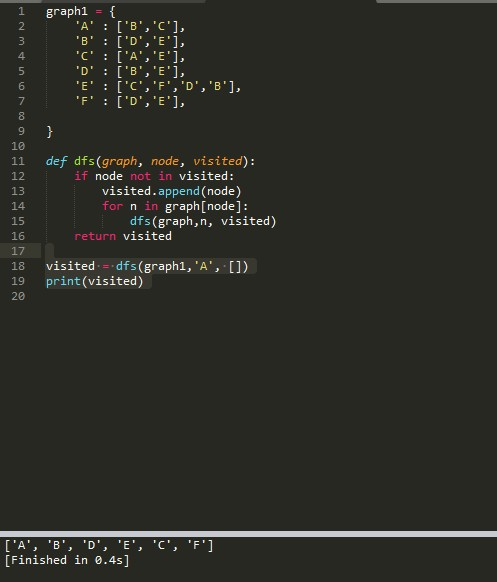
\includegraphics[width=35cm,height=16cm,keepaspectratio]{2.jpg}
\caption{Iplementation of Depth First Search}
\label{Figure:3}    
\end{figure*}
To traverse all the nodes in the graph using dfs technique.

\subsection{Procedure: Task 2 }     

\begin{lstlisting}[language=Python]


\end{lstlisting}

\section{Conclusion}  
In depth-first Search the memory requirement is only linear with respect to the search graph. This is in contrast with breadth-first search which requires more space. The reason is that the algorithm only needs to store a stack of nodes on the path from the root to the current node.So by traversing every node and backtracking where required we visited the whole tree.

 
\end{document}                          % The required last line
